%\documentclass[smallextended,referee]{svjour3}
%\documentclass[smallcondensed]{svjour3}
%\documentclass[smallextended]{svjour3}
\documentclass[referee]{svjour3}
\usepackage{lmodern,amsmath,graphicx}
%\usepackage[bibencoding=utf8,backend=biber,sorting=anyt]{biblatex}
%\usepackage[style=nejm,bibencoding=utf8,backend=biber,sorting=anyt]{biblatex}

\begin{document}
%\title{ Towards a universal MRI atlas of the prostate and prostate zones. Part II: Deep Learning }
\title{ Segmentation of prostate and prostate zones using Deep Learning: multiple MRI vendor analysis }

\author{
  Olmo Zavala-Romero$^1$ \and
  Adrian L. Breto$^1$ \and  
  Nicole Gautney$^1$ \and  
  Yu-Cherng C. Chang$^1$ \and 
  Alan Dal Pra$^1$ \and  
  Matthew C. Abramowitz$^2$ \and  
  Alan Pollack$^1$ \and  
  Radka Stoyanova$^1$
}

\institute{
    Olmo Zavala-Romero \at
    Department of Radiation Oncology, \\
    University of Miami Miller School of Medicine  \\
    1475 NW 12th Avenuew, Suite 1507, 
    Miami, FL 33136, USA\\
    Tel: (305)-243-2405\\
    E-mail: osz1@med.miami.edu
 }
\date{Received: date / Accepted: date}

\maketitle

\begin{abstract}
% 250 words
%Spacing of 1.5 lines, size 12 pt
A modified version of the 3D U-net  neural network architecture is used for automatic segmentation of the prostate and its peripheral zone (PZ) using multiplanar MRI. The network architecture is a multi-stream convolutional neural network (CNN) that uses axial, coronal, and sagittal MRI series as input.  A large dataset of 557 scans from multiple MRI vendors is used to analyze the consequences of training the CNN with distinct MRI magnets. The proposed segmentation scheme achieved good results for prostate and PZ compared to expert contoured volumes. Combining images from different MRI vendors on the training of the network is of paramount importance for training an universal model for prostate and peripheral zone segmentation. 

\keywords{ Prostate Cancer \and Multi-parametric MRI \and Deep Learning \and U-Net \and Machine Learning \and Prostate Zones}
\end{abstract}

% 2700 words without tables, captions and references.
\section{Introduction}
\label{sec:intro}
Accurate prostate segmentation on MRI datasets is required for many clinical and research 
applications. Furthermore, due to the different imaging properties of the peripheral (PZ) 
and transition zones (TZ) of the prostate, accurate zonal segmentation is also necessary. 
The prostate and zonal contours are necessary for computer aided diagnosis (CAD)
applications for staging, diagnosis, and treatment planning for prostate cancer. In 
a series of applications, prostate contours are fused with ultrasound images to
guide prostate biopsies. Automatic segmentation of the prostate, PZ and TZ on MR 
images provides an opportunity to broaden the current scope of research by facilitating 
studies that include large populations of subjects and/or studies that incorporate 
serial imaging of the prostate to grant a longitudinal picture of disease 
progression and response.  
Prostate MRI image segmentation has been an area of intense research \cite{litjens2014evaluation}. Earlier, the 
applied approaches varied from model-based \cite{chowdhury2012concurrent,toth2012multifeature},
 to atlas-based segmentation
\cite{4_klein2008automatic,5_cheng2014atlas, 6_xie2014low, 7_tian2015fully, 8_korsager2015use, 9_chilali2016gland}.
 Our group also evaluated the performance of atlas-based approach for prostate and prostate zones 
segmentation using data from different MR vendors and acquisition parameters\cite{10_padgett2018towards}. The advent 
of deep learning techniques, such as convolutional neural networks (CNN) has led to great success 
in image classifiation \cite{11_krizhevsky2012imagenet,12_simonyan2011immediate}. Recently, 
the U-Net architecture has been proposed \cite{13_ronneberger2015u} for medical imaging 
segmentation and has been applied to the prostate\cite{14_meyer2018automatic}.
In this work we present a modification of the U-Net architecture for segmentation of both 
the prostate and prostate zones. In continuation of our previous work for creating an 
universal segmentation tool, the network is evaluated for images from different MR vendors.  

\section{Methodology}
\label{sec:methods}
Met

\subsection{Preprocessing}
\label{subsec:prepro}
The preprocessing of the images include: automatic selection of a region
of interest, image resampling to a resolution of $0.5 x 0.5 x 0.5$ mm, contours interpolation
using optical flow, bias correction using the N4ITK algorithm \cite{n4itk}, and
image normalization to an interval of [0,1].

The selection of the region of interested was  

\section{Results}

Table \ref{tab:res_prost} shows the obtained DSCs for the segmentation of the prostate when the six trained models are used for the segmentation of the GE and Siemens dataset.  The displayed DSC is computed from the validation subset when the model is trained on the same dataset, and computed from the whole dataset when the model is trained from a different dataset. 
 \begin{table}[h]
    \label{tab:res_prost}
    \caption{Dice Similarity Coefficients between manual and CNN-generated prostate contours for GE and Siemens MRI vendors datasets. The trained models are divided in: with (w) data augmentation (DA) and without (wo) DA.}
    \begin{tabular}{lcc}
         \hline
          \textbf{Prostate Models} & \textbf{GE} & \textbf{Siemens }\\
         \hline
         %GE ROI/Original & $0.916\pm0.015$/$0.917\pm0.015$ & $0.465\pm0.198$/$0.466\pm0.198$ \\
         %GE & $\mathbf{0.917\pm0.015}$ & $0.466\pm0.198$ \\
         GE ROI/Original & $0.855\pm0.064$/$\mathbf{0.860\pm0.054}$ & $0.804\pm0.099$/$0.802\pm0.106$ \\
         \hline
         %Siemens ROI/Original & $0.261\pm0.119$/$0.276\pm0.130$ & $0.936\pm0.21$/$0.932\pm0.022$ \\
         %Siemens & $0.276\pm0.130$ & $\mathbf{0.932\pm0.022}$ \\
         Siemens ROI/Original & $0.262\pm0.118$/$0.288\pm0.139$ & $0.892\pm0.038$/$0.889\pm0.035$ \\
         \hline
         %Combined ROI/Original & $0.828\pm0.116$/$0.824\pm0.113$ & $0.909\pm0.032$/$0.907\pm0.031$\\
         %Combined & $0.824\pm0.113$ & $0.907\pm0.031$\\
         Combined ROI/Original & $0.830\pm0.112$/$0.827\pm0.109$ & $\mathbf{0.896\pm0.037}$/$0.892\pm0.036$\\
         \hline
    \end{tabular}
\end{table} 
When the model is trained with examples from one dataset and used to segment prostates from scans of the same MRI vendor the average DSCs are: 0.753 for GE and 0.893 for Siemens. When the datasets are combined during training, the average DSC are: 0.746 for GE and 0.909 for Siemens.  The results obtained for the Siemens dataset are comparable with current state of the art methods for prostate segmentation. When the model is trained with examples from one MRI vendor and then used to process images from a different vendor, the resulting DSCs are low (0.322 and 0.169).  %This result exhibit 
The above shows how sensible the model is to subtle changes in the training dataset. It also displays the importance of testing how well deep learning architectures generalize to other MRI vendors.  The use of data augmentation improves the generalization of the models in most cases but not with a clear tendency, further analysis is required.

Table \ref{tab:res_pz} shows the obtained DSCs for the segmentation of the PZ the six trained models.  The best DSCs (0.653 and 0.756) for segmenting the PZ of the prostate are obtained when the model is trained using the combined dataset.  
 \begin{table}[h]
    \label{tab:res_pz}
    \caption{Dice Similarity Coefficients (DSC) between manual and CNN-generated PZ contours for GE and Siemens.The trained models are divided in: with (w) data augmentation (DA) and without (wo) DA.}
    \begin{tabular}{lcc}
         \hline
          \textbf{PZ Models} & \textbf{GE Dataset} & \textbf{Siemens Dataset}\\
         \hline
         GE ROI/Original & $0.767\pm0.093$/$0.759\pm0.089$ & $0.537\pm0.204$/$0.539\pm0.204$ \\
         %GE  & $\mathbf{0.74\pm0.09}$ & $0.40\pm0.22$ \\
         \hline
         Siemens ROI/Original & $0.591\pm0.223$/$0.591\pm0.219$ & $0.808\pm0.085$/$0.808\pm0.087$ \\
         %Siemens & $0.58\pm0.21$ & $\mathbf{0.78\pm0.08}$ \\
         \hline
         Combined ROI/Original & $\mathbf{0.797\pm0.093}$/$0.788\pm0.093$ & $\mathbf{0.813\pm0.079}$/$0.811\pm0.79$\\
         %Combined & $0.75\pm0.10$ & $0.78\pm0.09$\\
         \hline
    \end{tabular}
\end{table}

The average DSCs of all the PZ models are lower than the coefficients for segmenting the prostate, which implies that PZ segmentation is a more challenging task.
Figure \ref{fig:resseg} shows one example of a prosate segmentation on the Siemens MRI vendor and a PZ segmentation on the GE MRI vendor. Both examples are from the middle layer of the prostate, and their corresponding DSC are 0.903 and 0.737.
 \begin{figure}[h]
    \centering
    \includegraphics[totalheight=.2\textheight]{figures/results/Prostate_Px_Challenge__P_yes_ROI_MIN_Case-0128.png}
    \includegraphics[totalheight=.2\textheight]{figures/results/Prostate_Px_Challenge__P_yes_ROI_MEAN_Case-0176.png}
    \includegraphics[totalheight=.2\textheight]{figures/results/Prostate_Px_Challenge__P_yes_ROI_MAX_Case-0337.png}
    \vspace{10mm}
    \includegraphics[totalheight=.2\textheight]{figures/results/Prostate_Px_Challenge__P_yes_Original_MIN_Case-0128.png}
    \includegraphics[totalheight=.2\textheight]{figures/results/Prostate_Px_Challenge__P_yes_Original_MEAN_Case-0085.png}
    \includegraphics[totalheight=.2\textheight]{figures/results/Prostate_Px_Challenge__P_yes_Original_MAX_Case-0016.png}
    \vspace{10mm}
    \includegraphics[totalheight=.2\textheight]{figures/results/Prostate_GE__GE_yes_ROI_MIN_Case-0518.png}
    \includegraphics[totalheight=.2\textheight]{figures/results/Prostate_GE__GE_yes_ROI_MEAN_Case-0544.png}
    \includegraphics[totalheight=.2\textheight]{figures/results/Prostate_GE__GE_yes_ROI_MAX_Case-0537.png}
    \vspace{10mm}
    \includegraphics[totalheight=.2\textheight]{figures/results/Prostate_GE__GE_yes_Original_MIN_Case-0518.png}
    \includegraphics[totalheight=.2\textheight]{figures/results/Prostate_GE__GE_yes_Original_MEAN_Case-0544.png}
    \includegraphics[totalheight=.2\textheight]{figures/results/Prostate_GE__GE_yes_Original_MAX_Case-0537.png}
    \label{fig:resseg}
    \caption{Prostate segmentations of Siemens (up) and GE (down) MRI vendors respectively. }
\end{figure} 

 \begin{figure}[h]
    \centering
    \includegraphics[totalheight=.2\textheight]{figures/results/PZ_Px_Challenge__P_yes_ROI_MIN_Case-0325.png}
    \includegraphics[totalheight=.2\textheight]{figures/results/PZ_Px_Challenge__P_yes_ROI_MEAN_Case-0319.png}
    \includegraphics[totalheight=.2\textheight]{figures/results/PZ_Px_Challenge__P_yes_ROI_MAX_Case-0026.png}
    \vspace{10mm}
    \includegraphics[totalheight=.2\textheight]{figures/results/PZ_Px_Challenge__P_yes_Original_MIN_Case-0325.png}
    \includegraphics[totalheight=.2\textheight]{figures/results/PZ_Px_Challenge__P_yes_Original_MEAN_Case-0319.png}
    \includegraphics[totalheight=.2\textheight]{figures/results/PZ_Px_Challenge__P_yes_Original_MAX_Case-0010.png}
    \vspace{10mm}
    \includegraphics[totalheight=.2\textheight]{figures/results/PZ_GE__GE_yes_ROI_MIN_Case-0481.png}
    \includegraphics[totalheight=.2\textheight]{figures/results/PZ_GE__GE_yes_ROI_MEAN_Case-0462.png}
    \includegraphics[totalheight=.2\textheight]{figures/results/PZ_GE__GE_yes_ROI_MAX_Case-0508.png}
    \vspace{10mm}
    \includegraphics[totalheight=.2\textheight]{figures/results/PZ_GE__GE_yes_Original_MIN_Case-0481.png}
    \includegraphics[totalheight=.2\textheight]{figures/results/PZ_GE__GE_yes_Original_MEAN_Case-0462.png}
    \includegraphics[totalheight=.2\textheight]{figures/results/PZ_GE__GE_yes_Original_MAX_Case-0508.png}
    \label{fig:ressegpz}
    \caption{PZ segmentations of Siemens (up) and GE (down) MRI vendors respectively. }
\end{figure} 

\section{Discussion/Conclusions}
\ref{sec:disc}
Manual contouring of the prostate requires slice-by-slice contouring 
in axial or in any of the other two views. Besides labor intensive, manual 
contouring is prone to inter-observer variability and imperfections 
in the 3D delamination (Figure 1). The U-net results in this paper show 
that in addition to efficiency and reproducibility, automatic prostate segmentation can be 
achieved with accuracy, similar to the expert’s manual contours reproducibility results. 


%\begin{acknowledgements}
%If you'd like to thank anyone, place your comments here
%and remove the percent signs.
%\end{acknowledgements}

\bibliographystyle{IEEEbib}
\bibliography{theref}
% Numbered in alphabetical order. Numbers in square brackets
%\printbibliography

\newpage
\textbf{Tables}
 \begin{table}[ht]
    \caption{Dice Similarity Coefficients (DSC) (mean \pm SD) for prostate, segmented with each of the three trained models (GE, Siemens, and Combined). The results are presented for data from GE and Siemens MRI vendors and the DSCs are calculated on the interpolated (0.5 x 0.5 x 0.5 mm) and original MRI resolution.}
    \begin{tabular}{lcc}
         \hline
          \textbf{Prostate Models} & \textbf{GE (Interpolated/Original Resolution)} & \textbf{Siemens (Interpolated/Original Resolution)}\\
         \hline
         GE & $0.855\pm0.064$/$\mathbf{0.860\pm0.054}$ & $0.804\pm0.099$/$0.802\pm0.106$ \\
         \hline
         Siemens & $0.262\pm0.118$/$0.288\pm0.139$ & $0.892\pm0.038$/$0.889\pm0.035$ \\
         \hline
         Combined & $0.830\pm0.112$/$0.827\pm0.109$ & $\mathbf{0.896\pm0.037}$/$0.892\pm0.036$\\
         \hline
    \end{tabular}
    \label{tab:res_prost}
\end{table} 

\newpage
\begin{table}[ht]
    \caption{Dice Similarity Coefficients (DSC) between manual and CNN-generated PZ contours for GE and Siemens.The trained models are divided in: with (w) data augmentation (DA) and without (wo) DA.}
    \begin{tabular}{lcc}
         \hline
          \textbf{PZ Models} & \textbf{GE Dataset} & \textbf{Siemens Dataset}\\
         \hline
         GE ROI/Original & $0.767\pm0.093$/$0.759\pm0.089$ & $0.537\pm0.204$/$0.539\pm0.204$ \\
         \hline
         Siemens ROI/Original & $0.591\pm0.223$/$0.591\pm0.219$ & $0.808\pm0.085$/$0.808\pm0.087$ \\
         \hline
         Combined ROI/Original & $\mathbf{0.797\pm0.093}$/$0.788\pm0.093$ & $\mathbf{0.813\pm0.079}$/$0.811\pm0.79$\\
         \hline
    \end{tabular}
    \label{tab:res_pz}
\end{table}

\newpage
\textbf{Figure legends:}
\begin{figure}[ht]
    \centering
    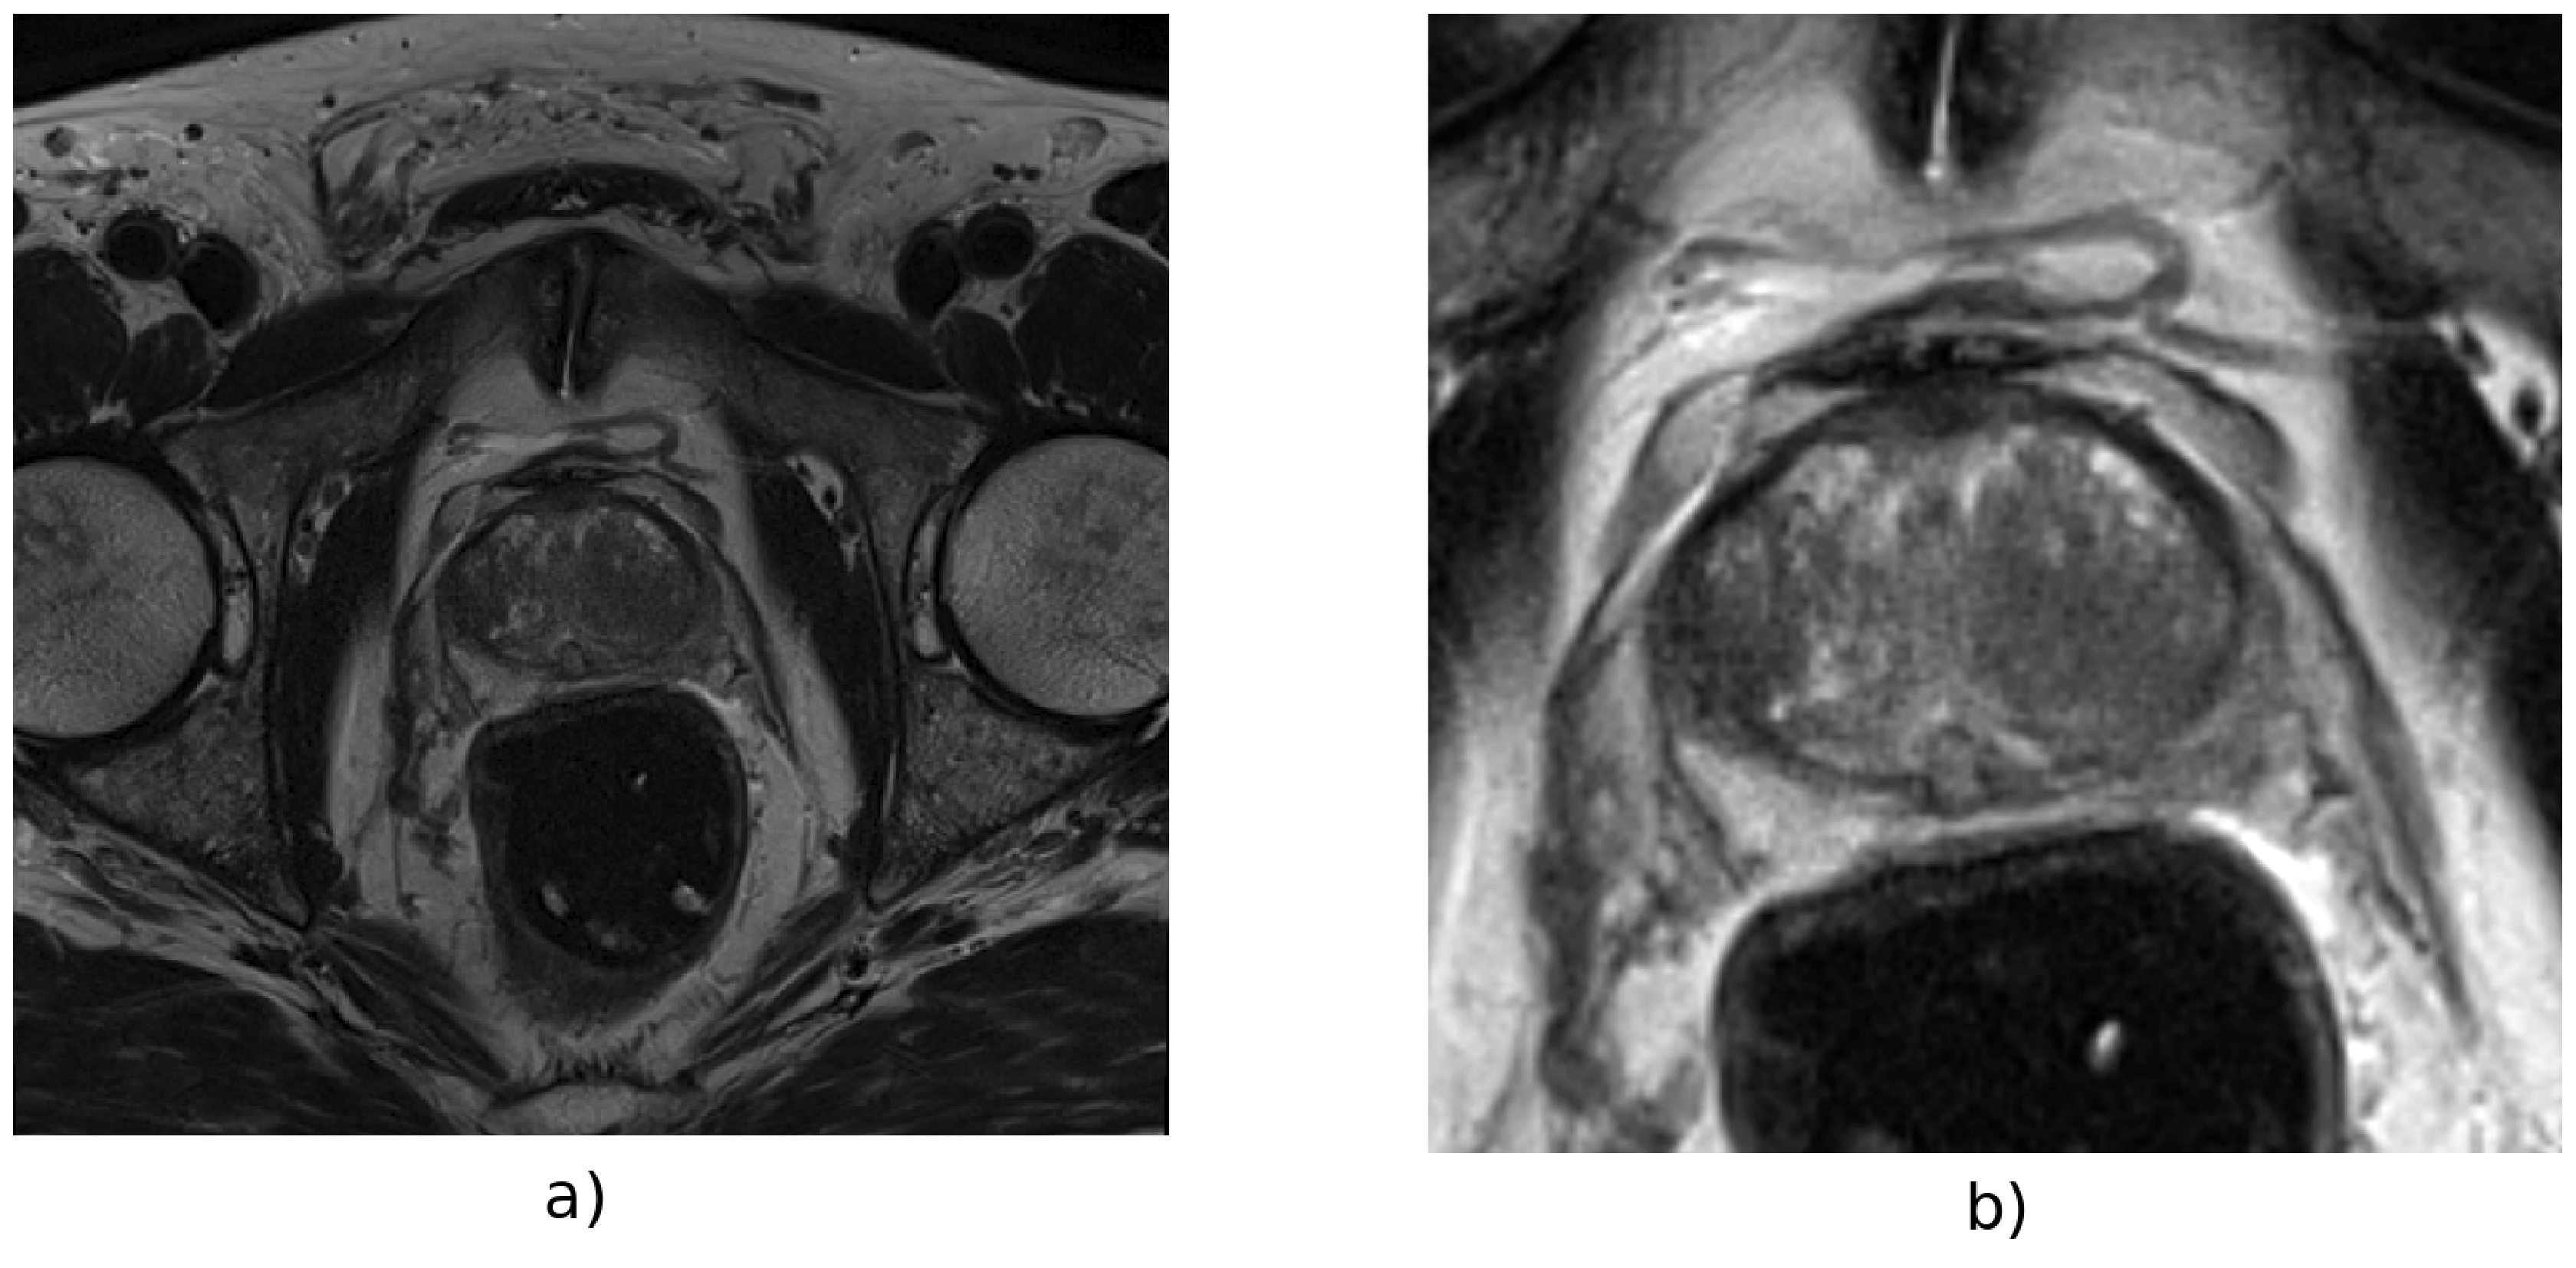
\includegraphics[totalheight=.25\textheight]{figures/Figure1.eps}
    \caption{The MRIs are preprocessed with bias correction, normalization, resampling, and cropped to a ROI to reduce the variability of sizes and intensities between magnets. In this example, \textbf{a)} is the original image and \textbf{b)} is the image after being processed.} 
    \label{fig_1}
\end{figure}

\begin{figure}[ht]
    \centering
    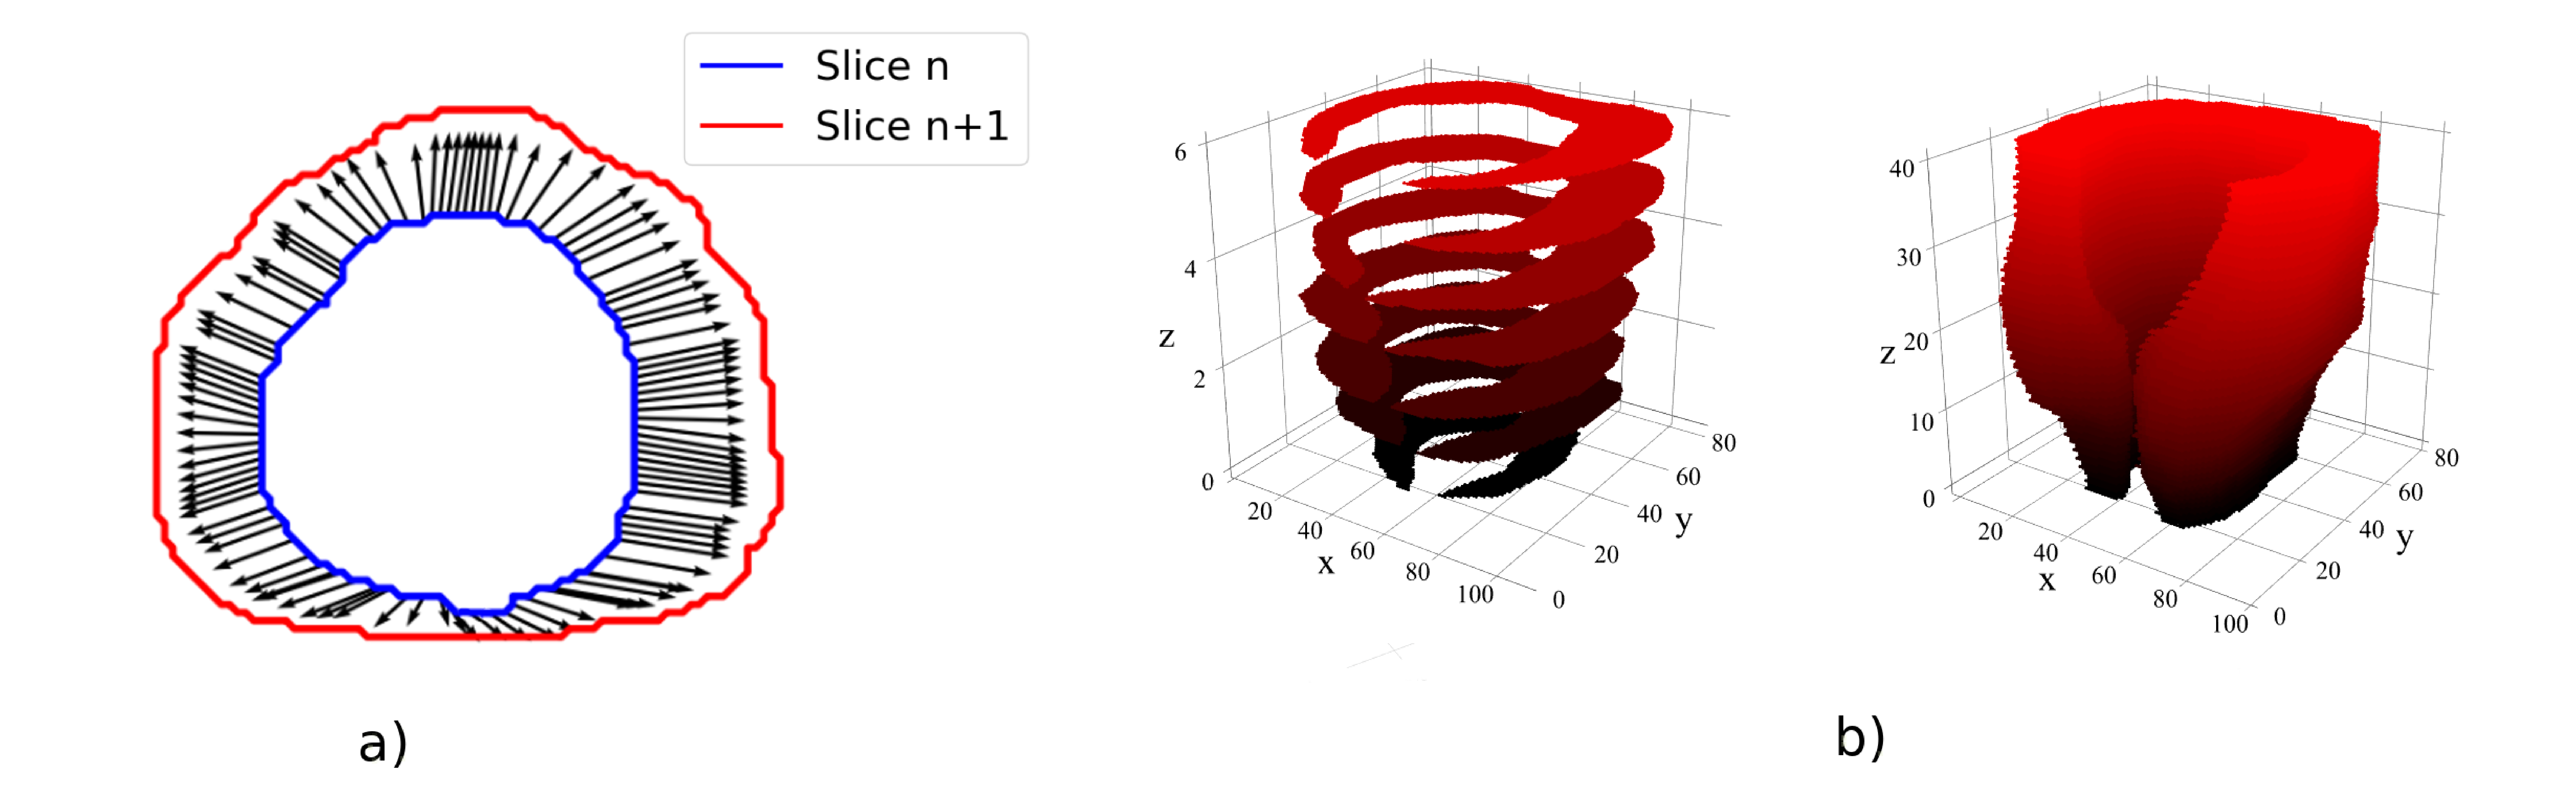
\includegraphics[totalheight=.21\textheight]{figures/Figure2.eps}
    \caption{Example of the proposed algorithm to increase the resolution of prostate and PZ contours. In \textbf{a)}, an example of the optical flow obtained between two prostate contours from adjacent horizontal planes. In \textbf{b)} on the left, original contours with 17 slices. On the right, interpolated contours with 68 slices.}
    \label{fig:fig_2}
\end{figure}

\begin{figure*}[ht]
    \centering
    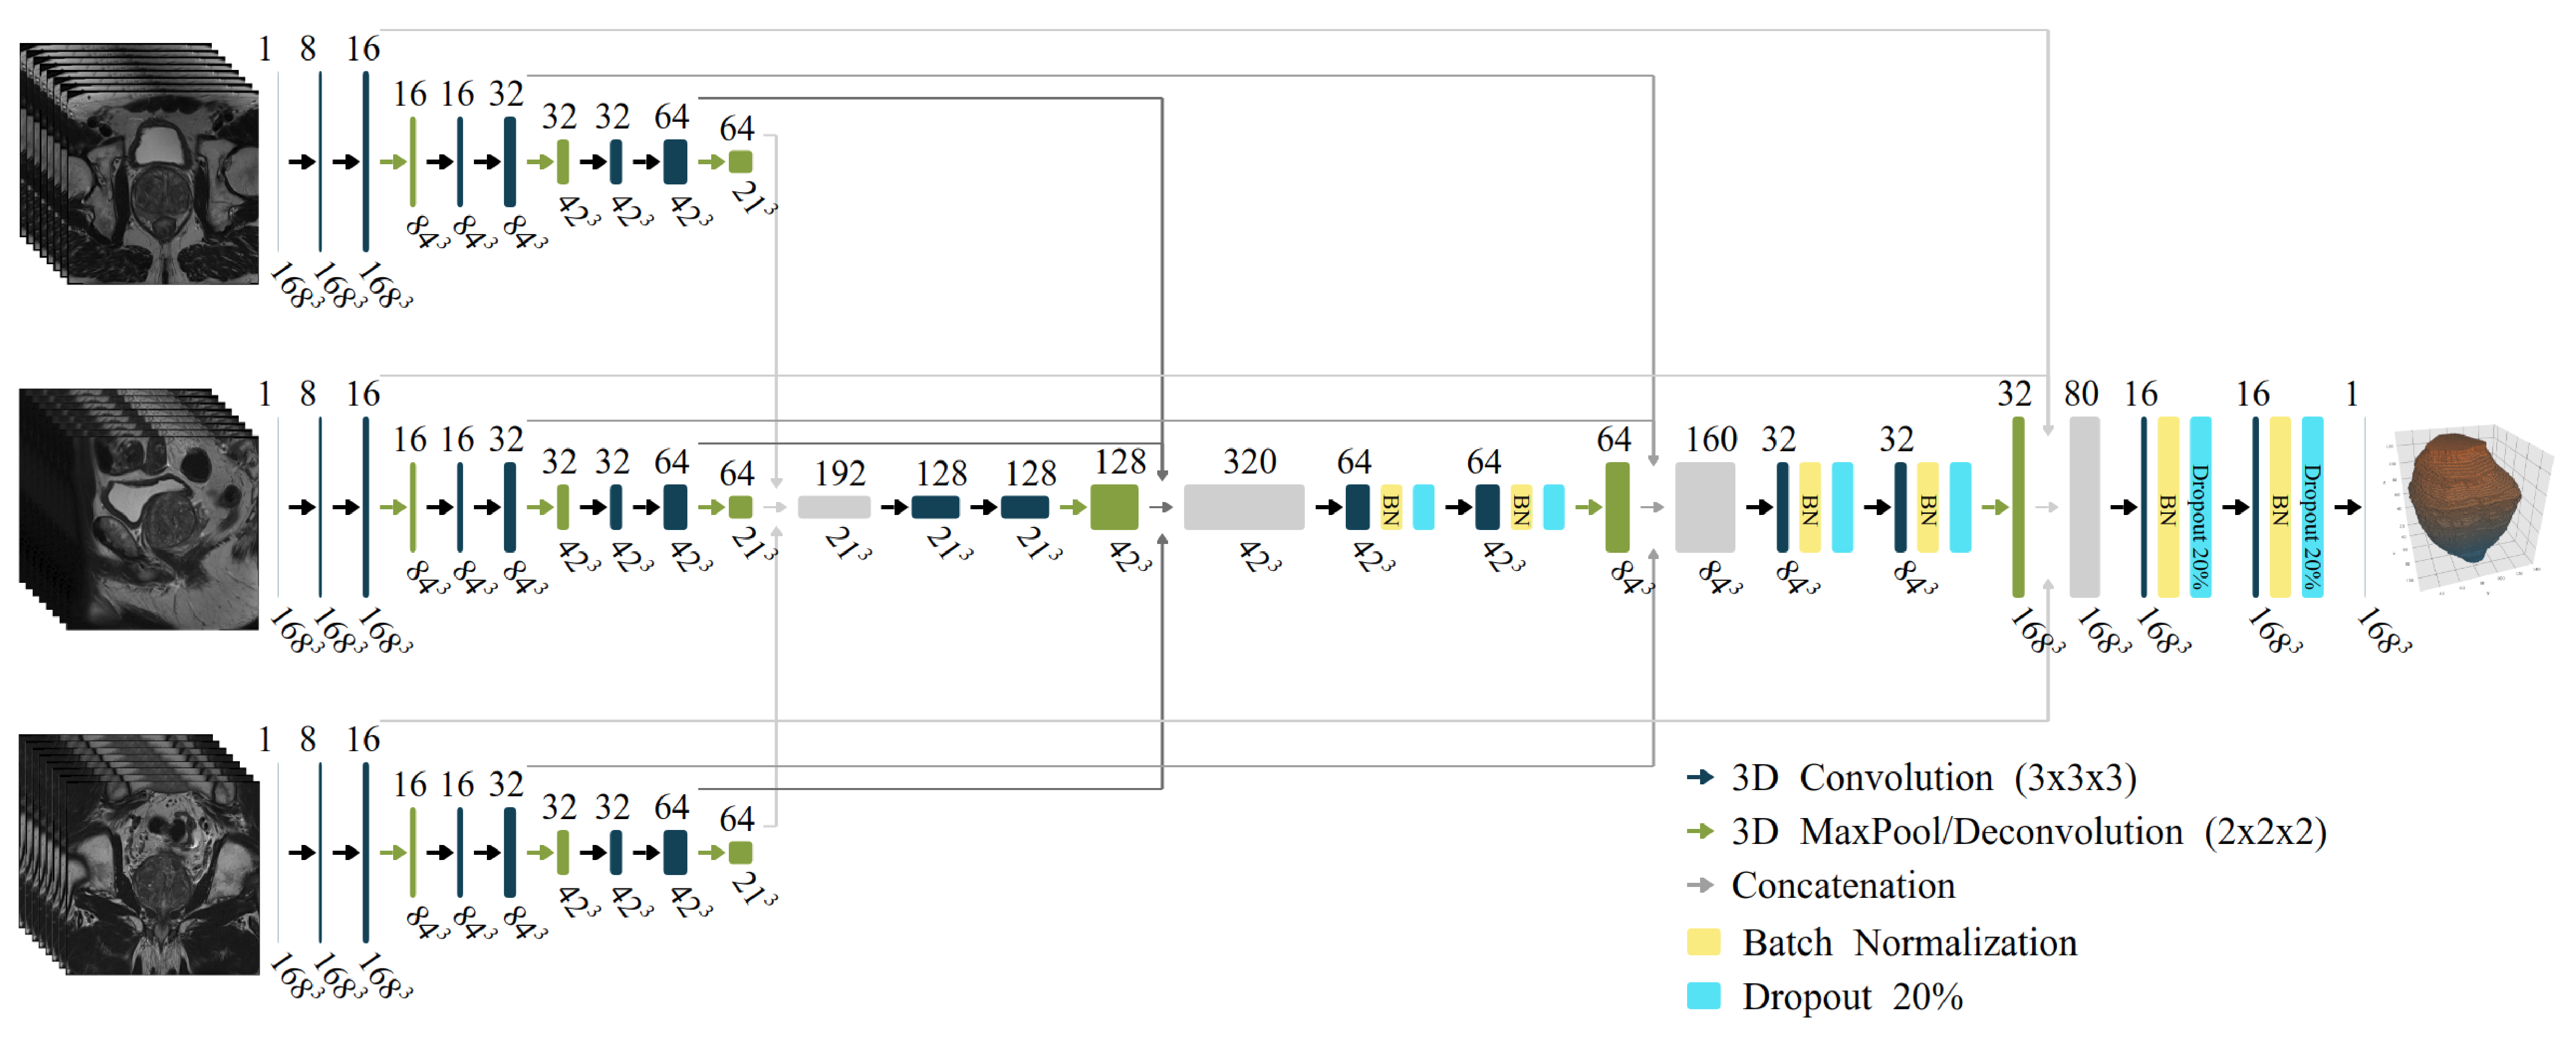
\includegraphics[totalheight=.282\textheight]{figures/Figure3.eps}
    \caption{Multistream 3D convolutional network architecture. The input of the network are three $168^3$ volumes from the MRI planes: axial, sagittal, and coronal. }
    \label{fig:fig_3}
\end{figure*}

\begin{figure}[ht]
    \centering
    \includegraphics[totalheight=.4\textheight]{figures/Figure4.eps}
    \caption{Prostate segmentation for the cases with the lowest, middle, and highest 3D DSC for the Siemens (up) and GE (down) datasets. These segmentation are obtained with the \emph{Combined} network model.  }
    \label{fig:resseg}
\end{figure} 

\begin{figure}[ht]
    \centering
    \includegraphics[totalheight=.4\textheight]{figures/Figure5.eps}
    \caption{Peripheral zone segmentation for the cases with the lowest, middle, and highest 3D DSC for the Siemens (up) and GE (down) datasets. These segmentation are obtained with the \emph{Combined} network model.  }
    \label{fig:ressegpz}
\end{figure} 

\end{document}
